% June 17
\chapter{Systemic Risk 1 - Fouque}
\section{History}
\begin{enumerate}
	\item 60's and 70's: 
	\begin{enumerate}
		\item Problem of Portfolio Allocation (Mean-Variance/Markovitz/)
		\item Option Pricing(1973) (Black-Scholes/etc)
	\end{enumerate}
	\item 90's:
	\begin{enumerate}
		\item Local Volatility
		\item Stochastic Volatility
	\end{enumerate}
	\item 2000's:
	\begin{enumerate}
		\item Credit - Taking into account the possibility of default(of company, counterparty, etc)
		\item Credit Basket - structuring risk(Mortgages)
		\item Credit Default Swap
		\item Collatorized Default Options - Huge Huge Market.
		\item Financial Crisis - Mortgages were completely mispriced.
	\end{enumerate}
	
	\item 2008-2010:
	\begin{enumerate}
		\item NIF: National Institute of Finance (for doing research on the banking \emph{system})
		\item Handbook on Systemic Risk: Cambridge
		\item Dodd-Frank: Created Office of Financial Research (under the treasury department)
	\end{enumerate}
\end{enumerate}

% \begin{definition}\label{def:systemic_risk}
% 	We define \emph{systemic risk}: 
% 	\begin{enumerate}
% 		\item a lot of defaults
% 		\item lack of liquidity
% 	\end{enumerate}
% \end{definition}

\section{Systemic Risk}
Can consider from many views: mathematics, statistics, etc.

Two main approaches:
\begin{enumerate}
	\item Coupled Diffusions: Continuous time
	\item Networks
\end{enumerate}

The starting point is Brownian Motion. Suppose we start with an asset:
\begin{equation}
	dS_t = \mu S_t dt
\end{equation}
which we can solve by
\begin{equation}
	S_t = S_0e^{\mu t}
\end{equation}
Okay, but usually we don't know the $\mu$, and there is some noise! How can we add noise? Since $\mu$ is the return, maybe by adding some \emph{white noise}
\begin{equation}
	dS_t = S_t(\mu dt + \text{Noise})
\end{equation}
where the Noise term is given by Brownian Motion, which has the form
\begin{equation}
	\sigma dW_t
\end{equation}
with $\sigma > 0$, and $(W_t)_{t\geq 0}$ for $t\leq T$. The properties of Brownian Motion:
\begin{enumerate}
	\item $W_0=0$
	\item $W_t$ is continuous
	\item Independent, increments
	\item If we consider
	\begin{equation}
		0 < t_1 < ... < t_n \leq T
	\end{equation}
	then it gives rise to many differences:
	\begin{equation}
		(W_{t_1} - W_{t_0}, W_{t_2} - W_{t_1}, ... W_{t_n} - W_{t_{n-1}})
	\end{equation}
	such that
	\begin{equation}
		\mathcal{D}(w_t - w_s) = \mathcal{N}(0, t-s)
	\end{equation}
\end{enumerate}
A bit of Brownian Motion History:
\begin{enumerate}
	\item Brown
	\item Buchelier (1900)
	\item Albert Einstein (1905): Heat Equation/Brownian Motion tie-in
	\item Weiner (1930s): Constructed Brownian Motion: Construct a measure over all continuous trajectories
	\item Ito (1940s): Figures out chain rule for brownian motion
	\item Samuelson (1960s): Generalized Brownian Motion
\end{enumerate}

If we have a bounded function $f(t)$ where
\begin{equation}
	\sum_{0}^T \left( f(t_{i+1}) - f(t_i) \right) < \infty
\end{equation}
If we have a brownian motion instead,
\begin{equation}
	\sum_0^T \left| W_{t_{i+1}} - W_{t_i} \right| \to \infty
\end{equation}

Book Reference: Carson \& Tree???

\section{Hitting Times}
Draw a plot:
\begin{enumerate}
	\item time on horizontal axis
	\item y = brownian motion on vertical axis
	\item line $y=\alpha$.
\end{enumerate}

\begin{figure}[htbp]
	\centering
		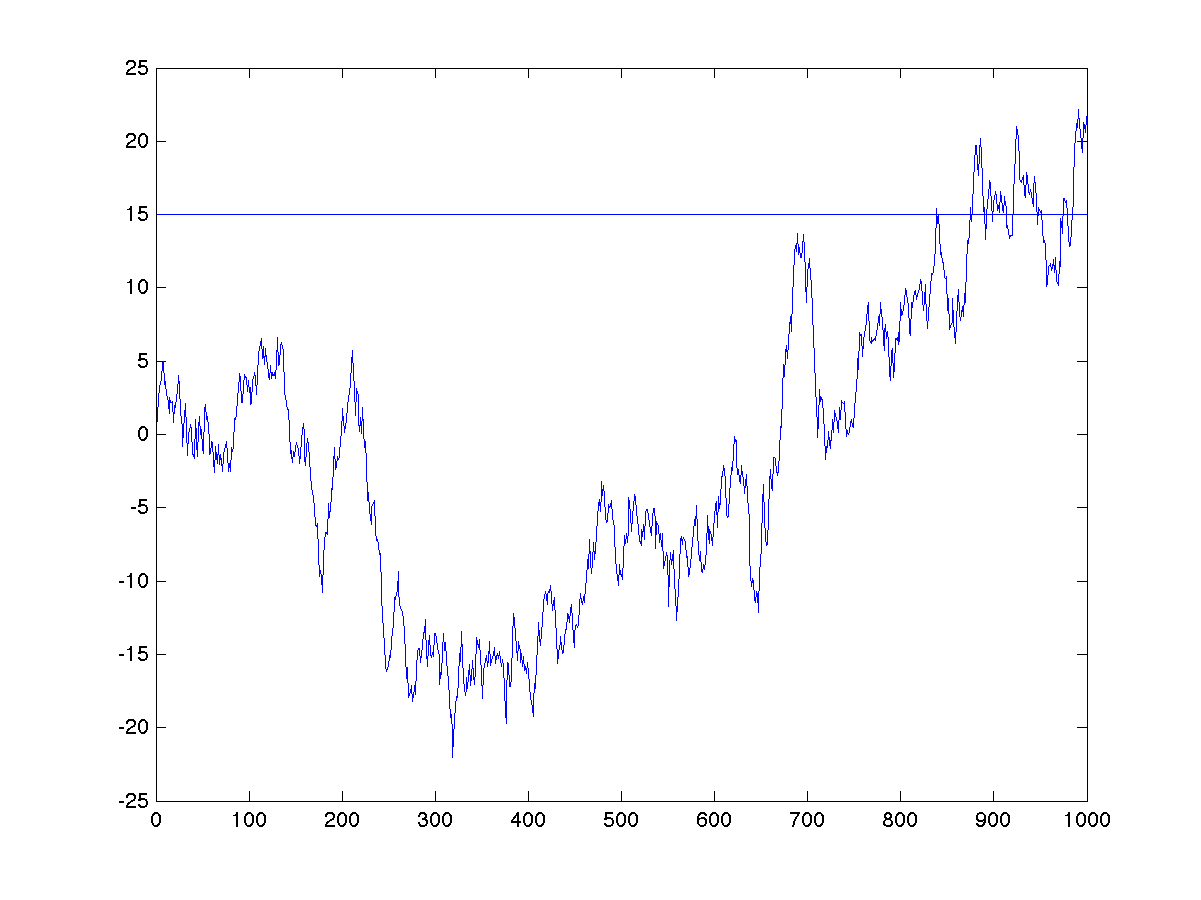
\includegraphics[width=.9\linewidth]{brownian_motion.png}
	\caption{caption}
	\label{fig:label}
\end{figure}

We are interested in the time $\tau_{\alpha}$, defined by
\begin{equation}
	\tau_a = \inf \{ t>0 : W_t \geq a \}
\end{equation}
(We are really looking for $W_t=a$)

We can instead think
\begin{equation}
	\{ \tau_a\leq t \} = \{ \max_{0\leq s \leq t} W_s \geq a \}
\end{equation}
Then
\begin{equation}
	\tilde{W}_t = W_t \Theta_{t \leq \tau} + (2a - W_t) \Theta_{t > \tau}
\end{equation}
is a Brownian Motion. RP.

Now suppose we want to find the probability:
\begin{align}
	\mathbb{P}(\tau& \leq t, |W_t-a|> b) \\
	=& \mathbb{P}(\tau \leq t, W_t > a+b) + \mathbb{P}(\tau \leq t, W_t < a-b)\\
	=& 2\mathbb{P}(\tau \leq t, W_t > a+b)\\
	=& 2N_{(0,t)}(-a-b)
\end{align}
But we also know that
\begin{equation}
	\mathbb{P}(\tau \leq t) = 2N_{(0,t)}(-a)
\end{equation}

A few remarks:
\begin{enumerate}
	\item $\tau$ is predictable. We say that $\tau$ is \emph{announced} by a sequence $\tau_n$, the hitting time of $a-\frac1n$.
	\item Large Deviations: Consider the probability of a very large deviation ($a \to \infty$)
	\begin{equation}
		\mathbb{P}(\tau_a \leq t) \sim e^{-\frac{a^2}{2t}}
	\end{equation}
	where we mean this in term of the log.
\end{enumerate}


\chapter{Systemic Risk 2 - Fouque}
\section{Joint Distributions}
Consider the joint distribution of $(\tau,W_t)$. We can think of this as
\begin{equation}
	``\mathbb{P}(\tau\leq t, W_t = v)'' = \begin{cases}
		\mathbb{P}(W_t = v) & \text{if } v > a\\
		\mathbb{P}(W_t=2a-v) & \text{if } v < a
	\end{cases} = \begin{cases}
		g(v)\\
		g(2a-v)
	\end{cases}
\end{equation}

For nonstandard Brownian Motions,
\begin{equation}
	X_t = x + \mu t + \sigma W_t
\end{equation}
And then
\begin{equation}
	\tau = \inf \{ t> 0, x_t \geq a \}
\end{equation}
So then,
\begin{align}
	x_t \geq a  \iff& (x+\mu t + \sigma W_t \geq a)\\
	\iff& \mu t + \sigma W_t \geq a-x\\
	\iff& \frac{\mu}{\sigma} t + w_t \geq \frac{a-x}{\sigma}
\end{align}
Define $\theta=\frac{\mu}{\sigma}$, and $\tilde{a}=\frac{a-x}{\sigma}$.

Then we have that
\begin{equation}
	W_t + \theta t \equiv W_t^\theta
\end{equation}
Then Girsanov's Thm is 
\begin{equation}
	M_t^\theta = e^{-\theta W_t - \frac{1}{2}\theta^2t}
\end{equation}
Then
\begin{equation}
	\mathbb{E}(M_t^\theta) = 1
\end{equation}
and
\begin{equation}
	\frac{dP^\theta}{dP}|_{f_x} = M^\theta_t
\end{equation}

We can show that $W_t + \theta t \equiv W_t^\theta$ is a brownian motion under $\mathbb{P}^\theta$. So next,
\begin{equation}
	\mathbb{E}^\theta \left( x / F_s\right) = \frac{1}{M^\theta_s} \mathbb{E}(X M^\theta_t / F_s) 
\end{equation}
Then we will be able to show
\begin{equation}
	\mathbb{E}^\theta \left( e^{iu(W_t^\theta - W_s^\theta)} \right) = e^{-\frac{\mu^2}{2}(t-s)}
\end{equation}
Why do we care about all of that? Well, we can do the following:
\begin{equation}
	\tau = \inf \{ t> 0, W_t^\theta \geq \tilde{a} \}
\end{equation}
Then
\begin{equation}
	\mathbb{P}(\tau \leq t) = \mathbb{E}(\Theta_{\tau \leq t}) = \mathbb{E}^\theta \equiv \left( \Theta_{\tau \leq t} \frac{d\mathbb{P}}{d\mathbb{P}^\theta} \right)
\end{equation}
We can use the joint distribution of $(\tau, W_t^\theta)$.
\begin{equation}
	= N( -\frac{a - x - \mu t}{\sigma \sqrt{t}}) + e^{\frac{2(a-x)\mu)}{\sigma^2}} N(-\left( \frac{a - x + \mu t}{\sigma \sqrt{t}}\right))
\end{equation}

\section{Geometric Brownian Motion}
Now consider
\begin{equation}
	dS_t = S_t (\mu dt + \sigma dW_t)
\end{equation}
which is a stochastic differential equation. We should think of this as a convient notation for something more complicated. Basically,
\begin{equation}
	S_t dW_t \to \int_0^t S_a dW_a
\end{equation}

We will use Ito's lemma which lets us do the chain rule with a brownian motion:
\begin{equation}
	dg(W_t) = g'(W_t) dW_t + \frac12 g''(W_t)dt
\end{equation}
where $g(t,W_t)$ is once differentiable in $t$ and twice differentiable in $W_t$. Then if we have
\begin{equation}
	dX_t = \varphi_t dt + \psi_t dW_t
\end{equation}
then
\begin{equation}
	dg(X_t)  = g'(X_t)dX_t + \frac{1}{2} g''(X_t)d\langle x\rangle_t
\end{equation}
Then an SDE like
\begin{equation}
	dX_t = b(t,X_t)dt + \sigma(t,X_t) dW_t
\end{equation}
has a solution like
\begin{equation}
	S_t = S_0 e^{(\mu - \frac{\sigma^2}{2})t} + \sigma W_t
\end{equation}

\section{Passage Time}
Now consider
\begin{equation}
	dS_t = S_t(\mu dt + \sigma dW_t) = S_t(r dt + \sigma(dW_t + \frac{\mu-r}{\sigma}dt))
\end{equation}
well then, $\mathbb{P}^*$: $e^{-rt}S_t$ is a martingale.

\section{Defaultable Bond}
Now we want to have a defaultable bond. The bond starts at $S_0$ and has a default value of $D$(if it touches $D$ before maturity time $T$ then we have no payout, otherwise get 1.) So then the price of the bond is
\begin{equation}
	\mathbb{P}^D_{(0,T)} = \mathbb{E}^*(\Theta_{\tau > T}) = \mathbb{P}^*(\tau > T).
\end{equation}
So now we consider
\begin{equation}
	\{ \inf_{0 < t \leq T} S_0 e^{(r- \frac{\sigma^2}{2})t + \sigma W_t} > 0 \} 
\end{equation}
By taking the logarithm, we get a nonstandard brownian motion, which we can evaluate. By some computation, we can get
\begin{equation}
	\mathbb{P}^\theta(0,T) = e^{-rT}\left[ N(d_2^+) - \left(\frac{S_0}{D} \right)^{1-\frac{2r}{\sigma^2}}N(d_2^-) \right]
\end{equation}
with
\begin{equation}
	d_2^{\pm} = \frac{\pm \log \frac{S_0}{D} + \left(r - \frac{\sigma^2}{2} \right)t}{\sigma \sqrt{t}}
\end{equation}

The main ingredients here were reflection principle and change of measure. Alternatively, one could do this completely with partial differential equations.

\section{Yield}
We can represent the yield by
\begin{equation}
	y(0,t) = -\frac{1}{T}\log \frac{\mathbb{P}^D(0,T)}{\mathbb{P}(0,T)}
\end{equation}

\subsection{Example}
Consider some bond $B_1$ with a 10\% default rate. This is too risky for index funds, and not risky enough for hedge fund.

A financial engineer will do this: Buy two bonds, $B_1$ and $B_2$ (both with 10\% default rate), then stack them. Now
\begin{enumerate}
	\item pays if 2 defaults: 0.99
	\item pays if 1 default: .8
\end{enumerate}
What's the problem? We assumed independence.

In credit, the main risk was correlation of default. This is not really computable.

Consider two processes $W_t^{(1)}$, $W_t^{(2)}$ and the hitting times $\tau^{(1)}$ and $\tau^{(2)}$ try and figure the probability $\mathbb{P}(z^{(1)} > T; z^{(2)}> T)$, well, it's hard to quantify. If 

\section{Systemic Risk}
Usually we will consider the log-capitalization of Banks, and in particular multiple banks:
\begin{equation}
	dX_t^i = \mu_t^i dt + \sigma^i dW_t^i.
\end{equation}
\subsection{Toy Model}
We can consider the drift of capitalization, which includes some coupling of the systems.
\begin{equation}
	dX^i_t = \frac{a}{N} \sum_{j\ne i} (X^j_t - X_t^i)dt + \sigma^i (\rho dW_t^\theta + \sqrt{1-\rho^2} dW_t^i)
\end{equation}
where the $W^i_t$ are independent.
What is the intuition here? That borrowing and lending goes on between the banks. This is related to flocking and swarming models.

What other mathematical model behaves this way(where we have randomness but also attraction)? ornstein uhlenbeck process:
\begin{equation}
	dY_t = a(m-y_t)dt + \sigma dW_t,
\end{equation}
which we know how to solve:
\begin{equation}
	Y_t = m + (y-m)e^{-at} + \sigma e^{-at} \int_0^t e^{as}dW_p
\end{equation}
And we know that this is $\mathcal{N}(m, \frac{\sigma^2}{2a})$.

Next step is:
\begin{equation}
	d(\frac{1}{N} \sum_{i=1}^N X_t^i ) = 0 dt + \sigma \rho dW_t^0 + \frac{\sigma\sqrt{1-\rho^2}}{N} \sum_{i=1}^N dW_t^i.
\end{equation}
Now consider if $X_0^i=x_0^i=0$, which gives
\begin{equation}
	\bar{x}_t = \frac{1}{N}\sum_{i=1}^N X_t^i = \sigma \rho W_t^0 + \frac{\sigma \sqrt{1-\rho^2}}{N} \sum_{i=1}^N W_t^i
\end{equation}
If we take $\rho=0$ for a second, then
\begin{equation}
	\bar{x}_T \sim \frac{\sigma}{\sqrt{N}}\tilde{W}_t
\end{equation}


\chapter{Systemic Risk Day 3}
We will continue considering the equation governing the log-capitalization of the banks
\begin{equation}
	dX_t^i = \frac{a}{N} \sum_{j=1}^N (x_t^j - x_t^i)dt + \sigma (\rho dW_t^0 + \sqrt{1-\rho^2} dW_t^i)
\end{equation}
where $W^0$, ..., $W^N$ are independent brownian motions and $a$ represents the speed of trading. We can further consider the mean over all these,
\begin{equation}
	\bar{X}_t = \frac{1}{N} \sum_{i=1}^N X_t^i
\end{equation}
which lets us write as
\begin{equation}
	d X_t^i = a (\bar{X}_t - X_t^i)dt + \text{Noise}
\end{equation}
where the mean is governed by
\begin{equation}
	d\bar{X}_t = \sigma\rho dW_t^0 + \frac{\sigma \sqrt{1-\rho^2}}{N}\sum_{i=1}^N dW_t^i
\end{equation}
Which is equivalent to [ed: is this true?]
\begin{equation}
	= \sigma \sqrt{\rho^2 - \frac{1-\rho^2}{N}}dB_t
\end{equation}
This gives rise to a flocking behavior--all the banks will follow the mean--at least as long as the mean is large.

Consider the case where $\rho=0$ which gives
\begin{equation}
	\frac{\sigma}{\sqrt{N}}dB_t.
\end{equation}
We will count a bank as defaulting when it hits some default amount $D<0$. We can consider the event
\begin{equation}
	\left\{ \min_{0\leq t \leq T} \bar{X}_t < D \right\}
\end{equation}
And in particular, we can calculate the probability of default,
\begin{equation}
	\mathbb{P}(\min_{0\leq t \leq T} \bar{X}_t < D) 
	= \mathbb{P}(\tau \leq t) 
	= 2\mathcal{N}(\frac{D\sqrt{N}}{\sigma\sqrt{T}})
	\sim e^{-\frac{D^2 N}{\sigma^2 T}}
\end{equation}

Another interesting regime: $\rho=0$. Then
\begin{equation}
	\bar{X}_t \sim \sigma \rho W_t^0
\end{equation}
and
\begin{equation}
	\mathbb{P}(\bar{\tau} \leq t) = 2 \mathcal{N}(\frac{D}{\sigma \rho \sqrt{T}})
\end{equation}
But this actually isn't too interesting.

Another one: $N\to \infty$ with $\rho=0$. We must be very careful here--taking $N\to\infty$ completely misses the systemic risk. That is because $\bar{X_t}\to 0$. But we could consider $N\to\infty$ but then reconsider with $N$ large but finite later. In this case, the $(X_t^i)$ become OUs, which are independent.  Then
\begin{equation}
	d X_t^i = -a X_t^i + \sigma dW_t^i
\end{equation}
and we need to find the hitting time of an OU(which is annoying, but possible).


\section{Other models}
\subsection{Garnier - Papanicolaou - Wang}
Here, we replace the hitting times with a double well potential.

That is, we create a double-well potential: $V(x) = a x^4 + b x^2$ (with $a>0$, $b<0$). Then the equation becomes
\begin{equation}
	dX_t^i = h V'(X_t^i) dt + a \sum_{j=1}^N (X_t^i - X_t^j) dt + \sigma dW^i_t
\end{equation}


\section{Games}
Work done with Carmona and Sun. We want the bank to be able to do something. To start, consider
\begin{equation}
	dX_t^i = \frac{a}{N} \sum_{j=1}^N (X_t^j - X_t^i)dt + \alpha_t^i dt + \text{Noise}
\end{equation}
Now to prevent the bank from borrowing infinite money, we must introduce a cost:
\begin{equation}
	J^i = \sum_{0}^T \frac{(\alpha_i^t)^2}{2} dt
\end{equation}
where we would of course minimize $J^i$. But now of course we must include an incentive--otherwise, we would just never borrow. So we modify to
\begin{equation}
	J^i = \sum_{0}^T (\frac{(\alpha_i^t)^2}{2} - q \alpha_t^i(\bar{X}_t - X_t^i) )dt
\end{equation}
But we would also like a convex optimization problem, so we change to
\begin{equation}
	J^i = \sum_{0}^T (\frac{(\alpha_i^t)^2}{2} - q \alpha_t^i(\bar{X}_t - X_t^i) + \frac{\epsilon}{2}(\bar{X}_t - X_t^i)^2)dt
\end{equation}
(We can think of this as a regulator imposing some extra cost if we get too far from the mean.) Finally, we would like to include some other cost at the very end, and also take the expectation, which gives:
\begin{equation}
	J^i = \mathbb{E} \left\{ \sum_{0}^T (\frac{(\alpha_i^t)^2}{2} - q \alpha_t^i(\bar{X}_t - X_t^i) + \frac{\epsilon}{2}(\bar{X}_t - X_t^i)^2)dt + \frac{c}{2}(\bar{X}_T - X_T^i)^2 \right\}
\end{equation}
We can not take $\epsilon$ too small, we must have $\epsilon \geq q^2$.

This looks like a Mean Field Game(MFG), pioneered Lions-Lasry for the $N\to\infty$ case. This is interesting--we pass to the limit to get an easier problem. Another approach is from Carmona-Delarue. But it turns out that we can solve this game for $N$ finite, via a dynamic programming approach.

We start with $\alpha_t^i = \phi^i(t,X_t)$. The dynamic programming approach means also introducing the quantities
\begin{equation}
	V^i(t,x) = \min \mathbb{E}_x \left( \int_t^T --\text{as above}-- + (\text{terminal cond}) | \mathcal{F}_t \right)
\end{equation}

This is governed by the Hamilton-Jacobi-Bellman (?) equation:
\begin{equation}
	\int \left\{ \partial_T V^i + \sum_{j=1}^N (a (\bar{x}-x^j)+ \alpha^i)\partial_{x_j}V^i 
	+
	\frac{\sigma^2}{2} \sum_j \sum_k \left( \rho^2 + (1-\rho)^2 \delta_{j,k}\right)
	+
	\frac{(\alpha^i)^2}{2} 
	- 
	q\alpha^i (\bar{x}-x^i) 
	+ 
	\frac{\epsilon}{2}(\bar{x}-x^i)^2
	\right\} = 0
\end{equation}
[Ed: there was a random $\partial_{x^j, x^k}V^i$ floating around here.. I think it goes after the $\delta_{jk})$ part?]
Also $\delta_{jk}$ is the Kronecker delta.
Because we want the infimum, we just take the gradient. And we want it with respect to $\alpha^i$ so
\begin{equation}
	\partial_{x^i} V^i + \alpha^i - q(\bar{\alpha} - x^i) = 0
	\implies
	\hat{\alpha}^i = -\partial_{x^i} V^i + q(\bar{\alpha} - x^i), \qquad i=1,..,N
\end{equation}
But this assumes that we know $V^i$, which we do not! So next we consider
\begin{equation}
	\partial_t V^i + \sum_{j=1}^N \left[ 
	(a + q)(\bar{x}- x^j) - \partial_{x_j} V^j
	\right] \partial_{x^j}V^i
	+
	\frac{\sigma^2}{2} \sum_j\sum_k \left[
	 \rho^2 + (1-\rho^2)\delta_{jk}
	\right]\partial_{x^j x^k} V^i
	+ \frac12(\epsilon-q^2)(\bar{x}-x^i)^2 + \frac12 (\partial_{x^i} V^i)^2
\end{equation}

We'll try an Ansatz here:
\begin{equation}
	V^i(t, x) = \frac{\varphi_t}{2} (\bar{x}-x^i)^2 + \mu_t
\end{equation}
and impose that
\begin{equation}
	V^i(T,x) \to \varphi_T = C, \mu_T = 0
\end{equation}
which gives
\begin{equation}
	\partial_{x^j} V^i = \varphi_t(\frac{1}{N} \delta_{ij}) (\bar{x} - x^i)
\end{equation}
and
\begin{equation}
	\partial_{x^j, x^k} V^i_t = \varphi_t (\frac{1}{N} - \delta_{ij})(\frac{1}{N} - \delta_{ik})
\end{equation}
which gives
\begin{align}
	\varphi_t' =& 2(a+q) \varphi_t + (1-\frac{1}{N^2})\varphi_t^2 - (\epsilon - q^2), \qquad \varphi_T = C\\
	\mu_t' =& -\sigma^2(1-\rho^2)(1-\frac{1}{N})\varphi_t, \qquad \mu_T = 0
\end{align}
which are x-independent terms! Hooray!

Let's solve it:
\begin{equation}
	\varphi_t = \frac{-(\epsilon - q^2)(\exp(\Delta(T-t)) - 1) - C(\delta^+ \exp(\Delta(T-t)) - \delta^-)}
			 {(\delta^-\exp(\Delta(T-t)) - \delta^+ ) - C(1 - \frac{1}{N^2})(\exp(\Delta(T-t))-1)}
\end{equation}
where
\begin{align}
	\Delta =& \delta^+ - \delta^-\\
	\delta^\pm =& -(a+q) \pm \sqrt{R}\\
	R =& (a+q)^2 + (1 - \frac{1}{N^2})(\epsilon - q^2) > 0
\end{align}

Where are we at here? First, we have
\begin{equation}
	\hat{\alpha}_t^i = (q + (1 + \frac{1}{N})\varphi_t)(\bar{X} - X_t^i)
\end{equation}
and also
\begin{equation}
	dX^i_t = \frac{a}{N} \sum_{j=1}^N (X_t^j - X_t^i)dt + ( \text{above...} )dt + \text{Noise}
\end{equation}

[ed] I missed one here.

Could do $T\to \infty$ because the terminal time is annoying. One option is to take $c=0$, and optimizing $\frac{1}{T}J_T^i$. Taking $T\to\infty$ mean the effective rate of borrowing and lending is
\begin{equation}
	\frac{-(\epsilon - q^2)}{\delta^-}
\end{equation}

We could also take $N\to\infty$, but this will be on Friday. Tomorrow will be a different approach and compare the two.



\chapter{Systemic Risk Day 4}
Consider
\begin{equation}
	dX_t^i = a(\bar{x}_t-x_t^i)dt + \sigma(\rho dW_t^0 + \sqrt{1-\rho^2}dW_t^i) + \alpha^i dt
\end{equation}
for $i=1,..,N$. One way to handle this is the ``open-loop feedback'' approach, which introduces
\begin{equation}
	J^i = \mathbb{E}\left\{ \int_0^T (\frac{\alpha^i}{2}) - q \alpha^i(\bar{x}_t-x_t^i) + \sum (\bar{x}_t - x_t^i)^2 )dt  + \frac{c}{2}(\bar{x}_T - x_t)^2 \right\}
\end{equation}
Another way is the dynamic programming approach where we introduce $V^i(t,x)$.
A more different way is the closed loop approach due to Pontugigin (spelling?).
This is also a Forward-Backward DE approach. It works by introducing a Hamiltonian for each player $i$:
\begin{equation}
	H^i(\vec{x}, \vec{y}^i, \vec{\alpha}      )
	=
	\sum_{k=1}^N (\alpha(\bar{x} - x^k) + \alpha^k)y^{ik} + \frac{1}{2} (\alpha^i)^2 - q \alpha^i(\bar{x}-x^i) + \frac{\epsilon}{2}(\bar{x}-x^i)^2
\end{equation}
Then imposing that for $k\ne i$, we have $\alpha^k = \alpha^k(t,x)$.
All of this becomes the stochastic differential equations
\begin{align}
	dX_i =& \frac{\partial H^i}{\partial y} dt \cdots \\
	dY_t^{i,j}=& -\frac{\partial H}{\partial x^j} dt + Z_t d\tilde{W}_t
	Y_T^{i,j} =& C(\bar{x}_T-x^i_T)(\frac{1}{N} - \delta_{ij})
\end{align}
So now we must calculate these Hamiltonian parts:
\begin{equation}
	\frac{\partial H^i}{\partial x^j} = 
	 \sum_{k=1}^N \left[ (a+q)(\frac{1}{N} - \delta_{kj} ) \right] y^{ik}
	 -q\alpha^i(\frac{1}{N} - \delta_{ij})
	 + \epsilon(\bar{x} - x^i) (\frac{1}{N} - \delta_{ij})
\end{equation}
and
\begin{equation}
	dY^{ij}_t = -\left[ \sum_{k=1}^N (a+y)(\frac{1}{N} - \delta_{kj})Y_t^{ik} - q\alpha^i(\frac{1}{N} - \delta_{ij}) + \sum (\bar{x}_t - x_t^i)(\frac{1}{N}-\delta_{ij})\right] dt + Z_t dW_t
\end{equation}
To solve, we take the anstaz
\begin{equation}
	Y_t^{ij} = \eta_t(\frac{1}{N}-\delta_{ij})(\bar{x}_t - x^i_t)
\end{equation}
Plug that in, then we get some expression for $dY_t^{ij}$.
Eventually, we get the differential equation from
\begin{equation}
	\eta_t' = 2(a + q)\eta_t + (1-\frac{1}{n^2})\eta_t^2 - (\epsilon - q^2), \quad \eta_T=C
\end{equation}

Okay, let's switch gears a bit and consider $N\to\infty$. Then $\bar{X}_t \to m_t$ is related to $\mathbb{E}(X^i_t/w^0)$
Then the one-player model ends up being
\begin{equation}
	dX_t = a (m_t - X_t)dt + \alpha_t dt + \sigma(\rho dW_t^0 + \sqrt{1-\rho^2}dW_t)
\end{equation}
So we will consider
\begin{equation}
	\inf \mathbb{E} \int_0^T \left( \frac{(\alpha_t)^2}{2} - q\alpha_t (m_t - X_t) + \frac{\epsilon}{2}(m_t - X_t)^2\right)dt + (other stuff)
\end{equation}
Then the Hamiltonian is
\begin{equation}
	H = \left[ \right] y + \frac{\alpha^2}{2} - q\alpha(m_t - x) + \frac{\epsilon}{2}(\mu_t-x)^2
\end{equation}
and again we'll set up the hamiltonians
\begin{align}
	dX_t = \frac{\partial H}{\partial y} dt + (noise)\qquad X_0=x_0\\
	dY_t = \frac{\partial H}{\partial x} dt + (noise)\qquad Y_T=(0 or TC)\\
\end{align}
Now then, because $\mathbb{E}(m_t - X_t)=0$, we have $\mathbb{E}(Y_t)=0$.
Using all of that, we can find $\mathbb{E}(X_t)= m_t $ (no surprise)
Then we get some equation like
\begin{equation}
	\alpha_t = - \eta_t X_t dt
\end{equation}
(but this equation is wrong, there is a $q$ somewhere)

Two references:
\begin{enumerate}
	\item Carmona-Delarue
	\item Mean Field Games: Lions-Cassry Cassy
\end{enumerate}

\chapter{Systemic Risk Day 5 \\ ???}

\section{Diversification vs Systemic Risk}
This will be an endogenous approach.

Consider two stocks $S^1$, $S^2$ which are geometric brownian motions.
Suppose they have mean growth $\mu$ and random part $\sigma$ and independent $W^1$, $W^2$.
We'll consider two banks with initial wealth $X^1_0=X^2_0=1$.
Consider the equations:
\begin{align}
	dX^1_t =& \mu X_t^1 dt + \sigma X_t^1 \left[(1-\alpha) dW^1_t  + \alpha dW^2_t \right]\\
	dX^2_t =& \mu X_t^2 dt + \sigma X_t^2 \left[\alpha dW^1_t  + (1-\alpha) dW^2_t \right]
\end{align}

Now consider $T>0$ with $\tau^1$, $\tau^2$ and default levels $D^1$, $D^2$. Then
\begin{equation}
	U^\alpha (t, x_1, x_2) = P(\tau_1> t, \tau_2 > t)
\end{equation}
Then the probability of a systemic event is
\begin{equation}
	P(\text{Systemic Event}) = 1+u^\alpha - u^{1,\alpha} - u^{2,\alpha}.
\end{equation}
There is a joint distribution of $\tau^1$, $\tau^2$. 
Then we can find a plot: Put $P(systemic)$ vs $\alpha$(the diversification parameter) The probability looks something like
\begin{equation}
	(1-u^1)(1-u^2)
\end{equation}
Then it is clear that there is some critical value $\alpha^c$.

Switching gears a bit, it is clear that $u^\alpha(t,x_1,x_2)$ satisfies a PDE:
\begin{equation}
	\partial_t u^\alpha  \cdots = 0 + T.C.  + B.C.
\end{equation}
(Insert plot: horizontal: $(0,T)$ , $x_1$ from some value to infinity, etc.)

\section{T. Ichibu Paper}
This is known as Feller's Diffusion (CIR) model:
\begin{equation}
	dX_t^i = \delta_i dt + \sum_{j=1}^n (x_t^j - x_t^i) p_{ij}(X_t)dt + 2\sqrt{X_t^i} dW^i_t
\end{equation}
with $X_t'$ is the capitalization.

\subsection{Quick review}
If we have
\begin{equation}
	dY^t = (m-Y_t)dt + \nu \sqrt{2 Y_t} dW^t
\end{equation}
then if $Y_0=0$ and if $\nu^2 \leq m$ (with $m>0$) then $Y_t>0 \forall t$.
(That is, the force of the process outweighs the volatility.)
The nice part of this is that it never hits zero.

We will need to solve an equation $\mathcal{L}u = 0$ of the form
\begin{equation}
	(m-y)u' + \nu^2 y u'' = 0
\end{equation}
which has a solution of the form
\begin{equation}
	u(y) = \int_1^y e^{\frac{z}{\nu^2}} z^{-\frac{m}{\nu^2}}dz
\end{equation}

Now consider a bound $[\epsilon, M]$. We are interested in the hitting time.
We can caluclate
\begin{equation}
	u(Y_{t \cap \tau}) = u(y) + \int_0^{t\cap \tau} u'(y_s) \nu \sqrt{2Y_s}dW_s
\end{equation}
The variance is given by
\begin{equation}
	\mathbb{E}( (u(y))^2) = u(y)^2 + \mathbb{E}\int_0^{t\cap \tau} u'(Y_s)^2 \nu^2 2 Y_s ds
\end{equation}
Then we have that
\begin{equation}
	\mathbb{E}(\tau) < +\infty \implies \tau < \infty \text{almost surely}
\end{equation}
Then we can do
\begin{equation}
	u(y) = \mathbb{E}(u(_\tau)) = u(\epsilon) P(\epsilon) + u(M)P(M)
\end{equation}
Now $u(\epsilon)\to -\infty$ and $P(\epsilon)\to 0$ as $n\to \infty$.

Next, if $\delta_i > 0$ and $P_{ij}$ bounded, regular enoguh, then there exists a solution (According to Bass-Perkins 2003).

We $S_t = \sum_{i=1}^n X_t^i$, and $P_{ij} = P_{ji}$, and we have the equation
\begin{equation}
	dS_t= (\sum_{i=1}^n \delta_i)dt + 2 \sum_{i=1}^n \sqrt{X_t} dW_t^i
\end{equation}
Equation: $\mathcal{D}$: $2 \sqrt{S_t} dB_t$.

Then we have
\begin{equation}
	dS_t = \left(\sum_{i=1}^n \delta_i \right)dt + 0 + 2\sum_{i=1}^n \sqrt{x^i_t} dW^i_t
\end{equation}
Which is equivalent to $\sqrt{S_t}dB_t$. Also, define
\begin{equation}
	\delta^* = \sum_{i=1}^n \delta_i
\end{equation}

This gives rise to a square Bessel process: $\delta^*\geq 2$; then $P(\tau < +\infty)=0$. If $\delta^*=2$ still $P(\tau<+\infty)=0$ but also $P(\limsup_t S_t = \infty)=1$ and $P(\inf_t S_t = 0)=1$. Next, consider $0 < \delta^* < 2$; Then $P(\tau<+\infty)=1$ via a reflecting principle. Finally, if $\delta^*=0$, then $0$ is absorbing.

\section{Multiple Defaults}
If for $(\ell_1,...,\ell_k) \subset \{ 1,2,..., n \}$,
\begin{equation}
	\sup_x \left|x_{\ell_i} - x_j \right| p_{\ell_i, j}(x) < 2c_0 = \frac{1}{h(h-1)} \left(2 - \sum_{i=1}^h \delta_{\ell_i} \right) 
\end{equation}
then we have that
\begin{equation}
	P(\exists t < +\infty s.t. X_t^{\ell 1}=...=X_t^{\ell_h}=0) = 1
\end{equation}
Can also show the converse.

We can show $P_{ij}=\frac{1}{n}$. We can then consider the mean field model:
\begin{equation}
	dX_t^i = \left( \delta_i + m - x_t^i \right) dt + 2 \sqrt{X_t^i }dW_t^i
\end{equation}
where
\begin{equation}
	\lim_{n\to \infty} \frac{1}{n} \sum_{i=1}^n X_0^i 
\end{equation}

Next, we could consider the health of a group of banks:
\begin{equation}
	\sum_{j=1}^n \sum_{i=1}^k \left( X_t^i - X_t^k \right)p_{k, j} (X_t)
\end{equation}

We could also create networks: Create a link between $i$ and $j$ if there is a certain amount of flow. Now we have a graph by looking at these quantities.
Then we can start asking questions about the size of the system, path lengths between banks, statistics of the system, etc.

\chapter{Rama Cont}
Bank balance sheets:
\begin{enumerate}
	\item Assets
	\begin{enumerate}
	\item Liquid Assets
	\item Interbank claims
		\item Other assets
	\end{enumerate}
	\item Liabilities
	\begin{enumerate}
		\item Deposits
		\item Interbank liabilities
		\item Short-term debt
		\item Capital
	\end{enumerate}
\end{enumerate}

Key parts: Solvency vs Liquidity.

\section{Microprudential approach}
Traditional approach to risk management and bank regulation is to focus on failure/non-failure solvency, liquidity) of individual banks. It focuses on the balance sheet structure of the individual banks.

They assume that losses arise due to exogenous random fluctuations in risk factors.
The main tool for stabilization of system is the capital requirements.
But it ignores links or interactions between market participants.

\section{Liability Chain}
Due to Hellwig. Consider a finite set of banks $i=1..N$, where
\begin{enumerate}
	\item $i$ borrows \$100 from $i-1$ over $i$ years
	\item $i$ lends \$100 to $i+1$ over $i+1$ years
\end{enumerate}

\chapter{Contagion and systemic risk in financial networks \\ Rama Cont}
Exposure networks: Let $E_{ij}$ denote exposure of $i$ to $j$.


























